% =============================================================================
% Block 2 --- Aula 2: Solow mechanics (per worker, no technological progress).
% Weighted toward Prova 01 error cluster 2 (carry the exponent; level versus growth effects).
\bloco{2}{The Solow model: mechanics}{Aula 2 \,\textbullet\, Kurlat ch.~3, \S4.1--4.2 \,\textbullet\, 10 points}

\questao{(4 points) \textit{Source: Kurlat, P. (2020), \emph{A Course in Modern Macroeconomics}, Exercise 4.2 ``The Black Death'',
pp.~72--73 --- statement reproduced verbatim, all items (a)--(d).}}

\noindent In the middle of the 14th century, a plague killed about a third of the population of Europe. Assume that the economy of Europe
was well described by the Solow model. How would the following variables change in response to the Black Death in the short run
(i.e.\ immediately)?
\begin{enumerate}[label=(\alph*),leftmargin=2.2em,topsep=2pt,itemsep=1pt]
\item GDP,
\item GDP per capita,
\item wages,
\item interest rates.
\end{enumerate}
\noindent\textit{Added parts (not in the book):} use $Y=AK^{\alpha}L^{1-\alpha}$; give each change as a factor and, with $\alpha=1/3$, as a
percentage. Then add one line per variable on the long run, with $s$, $n$, $\delta$ and $A$ unchanged.
\resolespaco
\begin{sol}
\begin{notacao}
\item $Y$, $K$, $L$: output, capital and population (= labour force). $A>0$: productivity. $\alpha\in(0,1)$: capital share, here $1/3$.
\item $k\equiv K/L$, $y\equiv Y/L$: capital and output per capita. $w$: real wage. $r^K$: rental rate of capital.
$r$: real interest rate. $\delta\in(0,1)$: depreciation. $s$, $n$: saving rate and population growth.
\item A prime marks a value just after the plague; $k^*$: the steady-state capital per capita.
\end{notacao}
\passo{model and prices}{The statement's technology, and its per-capita form (divide by $L$):}
\begin{align}
Y&=AK^{\alpha}L^{1-\alpha}, \label{b2q4:Y}\\
y&=Ak^{\alpha}. \label{b2q4:y}
\end{align}
Competitive factor prices are the marginal products of \eqref{b2q4:Y}:
\begin{align}
w&=\frac{\partial Y}{\partial L}=(1-\alpha)Ak^{\alpha}, \label{b2q4:w}\\
r^K&=\frac{\partial Y}{\partial K}=\alpha Ak^{\alpha-1},\qquad r=r^K-\delta. \label{b2q4:rK}
\end{align}
\passo{the shock}{On impact a third of the population dies and capital does not:}
\begin{equation}
\frac{L'}{L}=\frac23,\qquad \frac{K'}{K}=1,\qquad\text{so}\qquad \frac{k'}{k}=\frac32. \label{b2q4:shock}
\end{equation}
\passo{(a) GDP}{Divide \eqref{b2q4:Y} after the shock by \eqref{b2q4:Y} before, and use \eqref{b2q4:shock}:}
\begin{align*}
\frac{Y'}{Y}&=\frac{A(K')^{\alpha}(L')^{1-\alpha}}{AK^{\alpha}L^{1-\alpha}}\\
&=\Big(\frac{K'}{K}\Big)^{\alpha}\Big(\frac{L'}{L}\Big)^{1-\alpha}\\
&=(1)^{\alpha}\Big(\frac23\Big)^{1-\alpha}\\
&=\Big(\frac23\Big)^{2/3}=0.763 .
\end{align*}
GDP falls about $24\%$, less than the third of the population, because labour has diminishing returns.
\passo{(b) GDP per capita}{Using \eqref{b2q4:y} and \eqref{b2q4:shock}:}
\begin{align*}
\frac{y'}{y}&=\frac{A(k')^{\alpha}}{Ak^{\alpha}}\\
&=\Big(\frac{k'}{k}\Big)^{\alpha}=\Big(\frac32\Big)^{1/3}=1.145 .
\end{align*}
It \emph{rises} about $14.5\%$.
\passo{(c) wages}{Using \eqref{b2q4:w} and \eqref{b2q4:shock}:}
\begin{align*}
\frac{w'}{w}&=\frac{(1-\alpha)A(k')^{\alpha}}{(1-\alpha)Ak^{\alpha}}\\
&=\Big(\frac{k'}{k}\Big)^{\alpha}=\Big(\frac32\Big)^{1/3}=1.145 ,
\end{align*}
a rise of $14.5\%$.
\passo{(d) interest rate}{Using \eqref{b2q4:rK} and \eqref{b2q4:shock}:}
\begin{align*}
\frac{r^{K\prime}}{r^K}&=\frac{\alpha A(k')^{\alpha-1}}{\alpha Ak^{\alpha-1}}\\
&=\Big(\frac{k'}{k}\Big)^{\alpha-1}=\Big(\frac32\Big)^{-2/3}=0.763 .
\end{align*}
The rental rate falls about $24\%$, and by \eqref{b2q4:rK} $r=r^K-\delta$ falls by the same absolute amount.
\passo{long run}{$k'$ is above $k^*$, so saving per capita falls short of break-even investment, $sA(k')^{\alpha}<(n+\delta)k'$,
and $k$ falls back to the unchanged $k^*$. By \eqref{b2q4:y}--\eqref{b2q4:rK}, $y$, $w$ and $r$ return to their old values. $K$ and $Y$
converge to $\frac23$ of the path they would have followed: the population loss is permanent, its per-capita gain is
transitory.}
\intuicao{Labour became scarce relative to capital, so its marginal product rose and capital's fell; the survivors were richer
only until capital per worker depreciated back to the steady state.}
\refbib{Kurlat (2020), \S4.2 and \S4.4 (pp.~57, 63). The project's worked solution (Problem 4.2, folder
\texttt{Resolucao}) agrees on (a)--(c) but prints $0.874$ for (d), which is $(3/2)^{-1/3}$; the correct factor is $(3/2)^{-2/3}=0.763$.}
\rubrica{
\item 0.75 pt per item (a)--(d) with direction and factor; long run 1 pt. Wrong direction of $y$ or $w$ (thinking in totals): max.\ 0.25 pt in that item.
}
\end{sol}

% -----------------------------------------------------------------------------
\questao{(5 points) Discursive. \emph{Steady state $\times$ saving reform $\times$ convergence.} Per-worker variables throughout
($k=K/L$, $y=Y/L$, $c=C/L$). $Y_t=AK_t^{\alpha}L_t^{1-\alpha}$, $K_{t+1}=(1-\delta)K_t+sY_t$, $L_{t+1}=(1+n)L_t$, no technological
progress. Illustrative calibration for Brazil: $A=1$, $\alpha=1/3$, $s=0.20$, $n=0.02$, $\delta=0.08$.}

\textbf{a)} (2 points) Derive the law of motion of $k_t$ and find $k^*$, $y^*$ and $c^*$ in closed form in $(A,s,n,\delta,\alpha)$, then in
numbers. Use the limit $\alpha\to0$ to check the exponent of $y^*$.
\resolespaco
\begin{sol}
\begin{notacao}
\item $Y_t$, $K_t$, $L_t$: output, capital and workers in period $t$. $A>0$: productivity (constant). $\alpha\in(0,1)$: capital share.
\item $s\in(0,1)$: saving rate. $n\ge0$: labour-force growth. $\delta\in(0,1)$: depreciation.
\item $k_t\equiv K_t/L_t$, $y_t\equiv Y_t/L_t$, $c_t\equiv C_t/L_t$: per-worker capital, output and consumption.
$k^*$, $y^*$, $c^*$: their steady-state values.
\end{notacao}
\passo{the statement's equations}{Numbered here for reference:}
\begin{align}
Y_t&=AK_t^{\alpha}L_t^{1-\alpha}, \label{b2q5:Y}\\
K_{t+1}&=(1-\delta)K_t+sY_t, \label{b2q5:K}\\
L_{t+1}&=(1+n)L_t. \label{b2q5:L}
\end{align}
Dividing \eqref{b2q5:Y} by $L_t$ gives the per-worker technology:
\begin{equation}
y_t=Ak_t^{\alpha}. \label{b2q5:y}
\end{equation}
\passo{law of motion}{Divide \eqref{b2q5:K} by $L_{t+1}$, substitute \eqref{b2q5:Y} for $Y_t$ and \eqref{b2q5:L} for $L_{t+1}$:}
\begin{align}
k_{t+1}&=\frac{K_{t+1}}{L_{t+1}}\nonumber\\
&=\frac{(1-\delta)K_t+sAK_t^{\alpha}L_t^{1-\alpha}}{(1+n)L_t}\nonumber\\
&=\frac{(1-\delta)k_t+sAk_t^{\alpha}}{1+n}. \label{b2q5:lom}
\end{align}
\passo{steady state}{Set $k_{t+1}=k_t=k^*$ in \eqref{b2q5:lom} and multiply by $1+n$:}
\begin{align}
(1+n)k^*&=(1-\delta)k^*+sA(k^*)^{\alpha}\nonumber\\
(n+\delta)k^*&=sA(k^*)^{\alpha} \label{b2q5:be}\\
(k^*)^{1-\alpha}&=\frac{sA}{n+\delta}. \nonumber
\end{align}
Raise both sides to the power $1/(1-\alpha)$:
\begin{equation}
k^*=\Big(\frac{sA}{n+\delta}\Big)^{\frac1{1-\alpha}}. \label{b2q5:kss}
\end{equation}
Substitute \eqref{b2q5:kss} into \eqref{b2q5:y}:
\begin{align}
y^*&=A(k^*)^{\alpha}\nonumber\\
&=A\Big(\Big(\frac{sA}{n+\delta}\Big)^{\frac1{1-\alpha}}\Big)^{\alpha}\nonumber\\
&=A\Big(\frac{sA}{n+\delta}\Big)^{\frac{\alpha}{1-\alpha}}\nonumber\\
&=A^{\frac1{1-\alpha}}\Big(\frac{s}{n+\delta}\Big)^{\frac{\alpha}{1-\alpha}}. \label{b2q5:yss}
\end{align}
Consumption is the output not saved:
\begin{equation}
c^*=(1-s)\,y^*. \label{b2q5:css}
\end{equation}
\passo{numbers}{With $A=1$, $\frac1{1-\alpha}=\frac32$ and $\frac{\alpha}{1-\alpha}=\frac12$, the ratio is $s/(n+\delta)=0.20/0.10=2$.
Using \eqref{b2q5:kss}, \eqref{b2q5:yss} and \eqref{b2q5:css}:}
\begin{align*}
k^*&=\Big(\frac{0.20\times(1)}{0.02+0.08}\Big)^{3/2}\\
&=2^{3/2}=2.8284,\\
y^*&=(1)^{3/2}\Big(\frac{0.20}{0.02+0.08}\Big)^{1/2}\\
&=2^{1/2}=1.4142,\\
c^*&=(1-0.20)\times(1.4142)\\
&=0.8\times1.4142=1.1314.
\end{align*}
Check with \eqref{b2q5:be}: $sy^*=0.2\times1.4142=0.2828$ and $(n+\delta)k^*=0.1\times2.8284=0.2828$.
\passo{exponent check}{As $\alpha\to0$, \eqref{b2q5:y} gives $y=A$ whatever $k$ is, and \eqref{b2q5:yss} gives $y^*\to A$ because
$\alpha/(1-\alpha)\to0$. Writing $y^*=A(s/(n+\delta))^{1/(1-\alpha)}$, i.e.\ substituting $k^*$ without raising it to $\alpha$, would give
$y^*\to As/(n+\delta)$: impossible.}
\refbib{Kurlat (2020), \S4.2, eq.~(4.2.2) (p.~57).}
\rubrica{
\item Law of motion 0.5; $k^*$ 0.5; $y^*$, $c^*$ with the right exponents 0.5; numbers and check 0.5. Break-even $\delta k$ without $n$: max.\ 1 pt.
Exponent $1/(1-\alpha)$ on $y^*$ (the Prova~01 Q2(b) slip): max.\ 1 pt.
}
\end{sol}

\textbf{b)} (1.5 points) A pension reform raises $s$ to $0.25$ for good. Find the new $y^*$ and its percentage change, the growth of $k$
and $y$ in the first period after the reform, consumption on impact and in the new steady state, and the long-run growth rate of $y$.
Draw the Solow diagram.
\resolespaco
\begin{sol}
\begin{notacao}
\item Symbols as in (a). $s'=0.25$: the new saving rate. $k^{*\prime}$, $y^{*\prime}$, $c^{*\prime}$: the new steady state.
\item $k_0=k^*$, $y_0=y^*$: values in the reform period; $k_1$, $y_1$: values one period later.
\end{notacao}
\passo{new steady state}{Now $s'/(n+\delta)=0.25/0.10=2.5$. Using \eqref{b2q5:kss} and \eqref{b2q5:yss}:}
\begin{align*}
k^{*\prime}&=\Big(\frac{0.25\times(1)}{0.02+0.08}\Big)^{3/2}\\
&=2.5^{3/2}=3.9528,\\
y^{*\prime}&=(1)^{3/2}\Big(\frac{0.25}{0.02+0.08}\Big)^{1/2}\\
&=2.5^{1/2}=1.5811,\\
y^{*\prime}/y^*&=1.5811/1.4142=1.1180,
\end{align*}
a rise of $11.8\%$. Taking logs of \eqref{b2q5:yss}:
\begin{equation}
\ln y^*=\frac{1}{1-\alpha}\ln A+\frac{\alpha}{1-\alpha}\big[\ln s-\ln(n+\delta)\big]. \label{b2q5:lny}
\end{equation}
Only $\ln s$ changes in \eqref{b2q5:lny}, so
\[
\Delta\ln y^*=\frac{\alpha}{1-\alpha}\ln\frac{0.25}{0.20}=0.5\times\ln1.25=0.1116 :
\]
the elasticity of $y^*$ to $s$ is $\alpha/(1-\alpha)=0.5$.
\passo{first period}{Divide \eqref{b2q5:lom} by $k_t$:}
\begin{equation}
\frac{k_{t+1}}{k_t}=\frac{(1-\delta)+sAk_t^{\alpha-1}}{1+n}. \label{b2q5:ratio}
\end{equation}
At $k_0=2.8284$:
\[
k_0^{\alpha-1}=\big(2^{3/2}\big)^{-2/3}=2^{-1}=0.5 .
\]
Substitute this and $s'$ into \eqref{b2q5:ratio}:
\begin{align*}
\frac{k_1}{k_0}&=\frac{(1-0.08)+0.25\times(1)\times(0.5)}{1+0.02}\\
&=\frac{0.92+0.25\times0.5}{1.02}\\
&=\frac{1.045}{1.02}=1.0245 .
\end{align*}
$k$ grows $2.45\%$. By \eqref{b2q5:y}:
\begin{align*}
\frac{y_1}{y_0}&=\frac{Ak_1^{\alpha}}{Ak_0^{\alpha}}\\
&=\Big(\frac{k_1}{k_0}\Big)^{\alpha}=(1.0245)^{1/3}=1.0081 :
\end{align*}
$y$ grows $0.81\%$, then less every period, since $k_t^{\alpha-1}$ in \eqref{b2q5:ratio} falls as $k_t$ rises.
\passo{consumption}{On impact $k$, hence $y$, is unchanged, and \eqref{b2q5:css} with $s'$ gives}
\[
c=(1-0.25)\times1.4142=1.0607<1.1314 .
\]
In the new steady state, \eqref{b2q5:css} gives
\begin{align*}
c^{*\prime}&=(1-0.25)\times(1.5811)\\
&=0.75\times1.5811=1.1859>1.1314 .
\end{align*}
It pays off in the long run because $s$ is still below the golden-rule rate $\alpha=1/3$ (Block~3).
\passo{long run}{$y$ converges to $1.5811$ and stops growing: long-run growth of $y$ stays \textbf{zero}. A level effect, not a growth effect.}
\passo{diagram}{The saving curve $sAk^{\alpha}$ shifts up and its crossing with the break-even line $(n+\delta)k$, eq.~\eqref{b2q5:be},
moves from $k^*$ to $k^{*\prime}$.}
\begin{center}
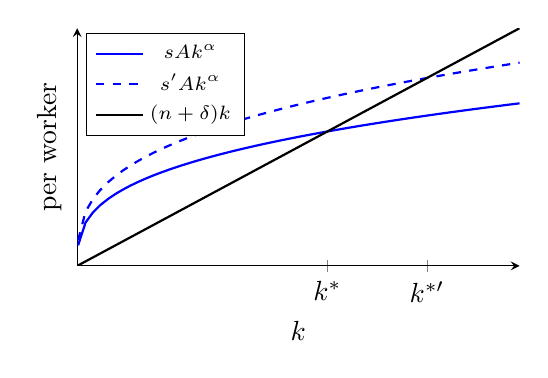
\begin{tikzpicture}
\begin{axis}[width=7.2cm,height=4.6cm,axis lines=left,xmin=0,xmax=5,ymin=0,ymax=0.5,xlabel={$k$},ylabel={per worker},
 xtick={2.828,3.953},xticklabels={$k^*$,$k^{*\prime}$},ytick=\empty,legend style={font=\scriptsize,at={(0.02,0.98)},anchor=north west},samples=60,domain=0.01:5]
\addplot[thick,blue]{0.20*x^(1/3)}; \addlegendentry{$sAk^{\alpha}$}
\addplot[thick,blue,dashed]{0.25*x^(1/3)}; \addlegendentry{$s'Ak^{\alpha}$}
\addplot[thick,black]{0.10*x}; \addlegendentry{$(n+\delta)k$}
\end{axis}
\end{tikzpicture}
\end{center}
\refbib{Kurlat (2020), \S4.2 (p.~57), Fig.~4.2.2.}
\rubrica{
\item $y^*$ and elasticity 0.5; first-period growth 0.5; consumption, long run and diagram 0.5. Saying long-run growth of $y$ rises: max.\ 0.5 pt.
Diagram without labelled curves or without the upward shift: $-0.25$ pt.
}
\end{sol}

\textbf{c)} (1.5 points) Two states share the calibration of (a): S\~ao Paulo sits at $k^*$ and Piau\'i starts at $k^*/8$. Find each state's growth
of $k$ and $y$ in the first period. Then let Piau\'i save only $s=0.10$: find its own steady state and its first-period growth, and say what
happens to $y_{PI}/y_{SP}$. Which kind of convergence does each case illustrate?
\resolespaco
\begin{sol}
\begin{notacao}
\item Symbols as in (a). $k_{PI}$, $y_{PI}$ and $k_{SP}$, $y_{SP}$: capital and output per worker in Piau\'i and S\~ao Paulo.
\item $s_{PI}=0.10$: Piau\'i's lower saving rate in the second case. $k^*_{PI}$, $y^*_{PI}$: its own steady state.
\end{notacao}
\passo{same parameters}{Piau\'i starts at $k_{PI}=2.8284/8=0.3536$. The term of \eqref{b2q5:ratio} that moves is}
\begin{align*}
k_{PI}^{\alpha-1}&=\Big(\frac{k^*}{8}\Big)^{-2/3}\\
&=(k^*)^{-2/3}\,8^{2/3}\\
&=0.5\times4=2 .
\end{align*}
Substitute into \eqref{b2q5:ratio} with $s=0.20$:
\begin{align*}
\frac{k_1}{k_0}&=\frac{(1-0.08)+0.20\times(1)\times(2)}{1+0.02}\\
&=\frac{0.92+0.20\times2}{1.02}\\
&=\frac{1.32}{1.02}=1.2941 .
\end{align*}
$k$ grows $29.4\%$; by \eqref{b2q5:y}, $y$ grows $1.2941^{1/3}-1=8.97\%$. S\~ao Paulo sits at $k^*$, where \eqref{b2q5:be} makes
\eqref{b2q5:ratio} equal to 1: it grows $0\%$. By \eqref{b2q5:y}, $y_{PI}=0.3536^{1/3}=2^{-1/2}=0.7071$ against $1.4142$: the poorer state
grows faster and the gap closes. Absolute convergence holds because both states share one steady state.
\passo{lower saving}{Piau\'i's own steady state: $s_{PI}/(n+\delta)=0.10/0.10=1$, so \eqref{b2q5:kss} and \eqref{b2q5:yss} give
$k^*_{PI}=y^*_{PI}=1$. At $k=0.3536$, \eqref{b2q5:ratio} with $s_{PI}$ gives}
\begin{align*}
\frac{k_1}{k_0}&=\frac{(1-0.08)+0.10\times(1)\times(2)}{1+0.02}\\
&=\frac{0.92+0.10\times2}{1.02}\\
&=\frac{1.12}{1.02}=1.0980 ,
\end{align*}
so $k$ grows $9.80\%$ and $y$ grows $1.0980^{1/3}-1=3.17\%$. It still grows, but toward its own lower level:
\[
\frac{y_{PI}}{y_{SP}}\ \text{rises from}\ \frac{0.7071}{1.4142}=0.5\ \text{to}\ \frac{1}{1.4142}=0.7071
\]
and stays there. Conditional convergence: growth depends on the distance from one's own steady state.
\intuicao{Diminishing returns make capital most productive where it is scarce; whether the poor catch up fully depends on
whether they share the rich economy's $s$, $n$, $\delta$ and $A$.}
\refbib{Kurlat (2020), \S3.3 (pp.~47--51) and Exercise~3.3 (p.~52); Exercise~5.2 (p.~94) on the speed of convergence.}
\rubrica{
\item Same-parameter growth rates 0.5; own steady state and growth 0.5; ratio and the absolute/conditional label 0.5.
Absolute convergence claimed for the low-saving case: max.\ 0.5 pt.
}
\end{sol}

% -----------------------------------------------------------------------------
\questao{(1 point) Multiple choice. Brazil's demographic transition lowers population growth $n$ from 2\% to 1\% a year for good. In
the Solow model without technological progress, starting and ending in steady state:}
\begin{alternativas}
\item $k^*$ and $y^*$ rise; long-run growth of $y$ stays at zero, while total GDP growth falls from 2\% to 1\% a year.
\item $k^*$ and $y^*$ rise; long-run growth of $y$ rises by one point, while total GDP growth stays at 2\% a year.
\item $k^*$ and $y^*$ fall; long-run growth of $y$ stays at zero, while total GDP growth stays at 2\% a year.
\item $k^*$ and $y^*$ rise; long-run growth of $y$ stays at zero, while total GDP growth stays at 2\% a year.
\item $k^*$ rises and $y^*$ stays put; long-run growth of $y$ stays at zero, while total GDP growth falls from 2\% to 1\% a year.
\end{alternativas}
\gabarito{A}
\begin{sol}
\begin{notacao}
\item Symbols as in Question~5; $g_Y$, $g_y$: growth rates of total GDP $Y$ and of GDP per worker $y=Y/L$.
\end{notacao}
\passo{levels}{By \eqref{b2q5:kss} and \eqref{b2q5:yss}, $k^*$ and $y^*$ both rise when $n$ falls: less investment goes to equipping new workers.}
\passo{growth}{Since $Y=yL$,}
\begin{equation}
1+g_Y=(1+g_y)(1+n). \label{b2q6:gY}
\end{equation}
In steady state $y$ is constant, $g_y=0$; substituting into \eqref{b2q6:gY}:
\begin{align*}
1+g_Y&=(1+0)(1+n)\\
g_Y&=n:
\end{align*}
total GDP growth falls from 2\% to 1\%. B confuses level with growth and
per capita with total (two mistakes); C gets the sign wrong and keeps total growth at 2\% (two); D keeps total growth at 2\%; E forgets that
$y^*=A(k^*)^{\alpha}$ moves with $k^*$.
\refbib{Kurlat (2020), \S4.2 (p.~57) and \S4.4 (p.~63).}
\end{sol}
